\documentclass{article}
\usepackage{listings}
\usepackage[a4paper, total={6in, 8in}]{geometry}
\usepackage{graphicx}

\title{CMOR 421/521, Homework \#1: \LaTeX{} Submission}
\author{\texttt{amc50}}
\date{February 29, 2024}

\begin{document}
\maketitle

\section{Compilation}

\subsection{Accessing NOTS Cluster}
\begin{verbatim}

It is important to note that the following process is done on Rice Owls
Network. If this is not the case, this would be unsucessful. 

Command used to ssh into NOTS:
MacBook-Pro-95:cmor-421-521-submissions antoniocrivello$ ssh amc50@nots.rice.edu

Command used to activate interactice node on NOTS:
[amc50@nlogin1 ~]$ srun --pty --partition=interactive --ntasks=1 --mem=1G --time=00:30:00 $SHELL

Command used to load modules needed for compilation:
[amc50@bc9u7n1 ~]$ module load GCC/13.1.0         

Accessing files on local desktop by using GitHub Repository:
[amc50@bc9u7n1 ~]$ ssh-keygen -t ed25519 -C "amc50@rice.edu"
\begin{comment}
Generating public/private ed25519 key pair.
Enter file in which to save the key (/home/amc50/.ssh/id_ed25519): 
Enter passphrase (empty for no passphrase): 
Enter same passphrase again: 
Your identification has been saved in /home/amc50/.ssh/id_ed25519.
Your public key has been saved in /home/amc50/.ssh/id_ed25519.pub.
The key fingerprint is:
SHA256:1Xu4gV32DaSy0mP1qHGao7fMWMgxI6UWWx7PYAILwSY amc50@rice.edu
The key's randomart image is:
+--[ED25519 256]--+
| .o..         .  |
|E o. o     . o   |
| o  . o * o + +  |
|       X B * B o.|
|      = S X B o o|
|     . o B B +   |
|        o * .    |
|         *..     |
|        o.+.     |
+----[SHA256]-----+
\end{comment}

Command used to access public key:
[amc50@bc9u7n1 ~]$ emacs ~/.ssh/id_ed25519.pub 

The key was then added to list of SSH Keys on GitHub.

Command used to clone cmor-421-521-submission GitHub repository:
[amc50@bc9u7n1 ~]$ git clone git@github.com:AntonioCrivello/cmor-421-521-submissions.git

\begin{comment}
Cloning into 'cmor-421-521-submissions'...
Warning: Permanently added the ECDSA host key for IP address '140.82.114.3' to the list of known hosts.
\end{comment}

For compilation on the NOTS Cluster I am utilizing a Makefile.
[amc50@bc9u7n1 homework-1]$ make clean
rm -f matmul_recursive ./obj/*.o *~ *.o

[amc50@bc9u7n1 homework-1]$ make
g++ -c src/matrix.cpp -o obj/matrix.o -I./include -O3 -std=c++11
g++ obj/matrix.o main.cpp -I./include -O3 -std=c++11 -o matmul_recursive

In order to efficiently generate timings for matrix sizes of 2^i for i = 4,5,6 ... 10
I have also created a bash script that runs the executable with the changing matrix size as the argument. 

[amc50@bc9u7n1 homework-1]$ ./generate-timings.sh 

\end{verbatim}

\section{Matrix-Matrix Multiplication}
\begin{verbatim}

    a
    
\end{verbatim}

\section{Optimizing Matrix-Matrix Multiplication}
\begin{verbatim}
\end{verbatim}

\subsection{Timing}
    \begin{table}[ht!]
        \begin{flushleft}
        \caption{Blocked Matrix-Matrix Multiplication on NOTS}
        \begin{tabular}{|c|c|c|}
            \hline
            & Number of Iterations & NOTS Timing \\
            \hline
            Matrix 4 x 4 & & \\
            \hline
            Matrix 8 x 8 & & \\
            \hline
            Matrix 16 x 16 & & \\
            \hline
            Matrix 32 x 32 & & \\
            \hline
            Matrix 64 x 64 & & \\
            \hline
            Matrix 128 x 128 & & \\
            \hline
            Matrix 256 x 256 & & \\
            \hline
            Matrix 512 x 512 & & \\
            \hline 
            Matirx 1024 x 1024 & & \\
        \end{tabular}
    \end{flushleft}
\end{table}

\subsection{Results}

\begin{figure}[!htb]
    \centering
    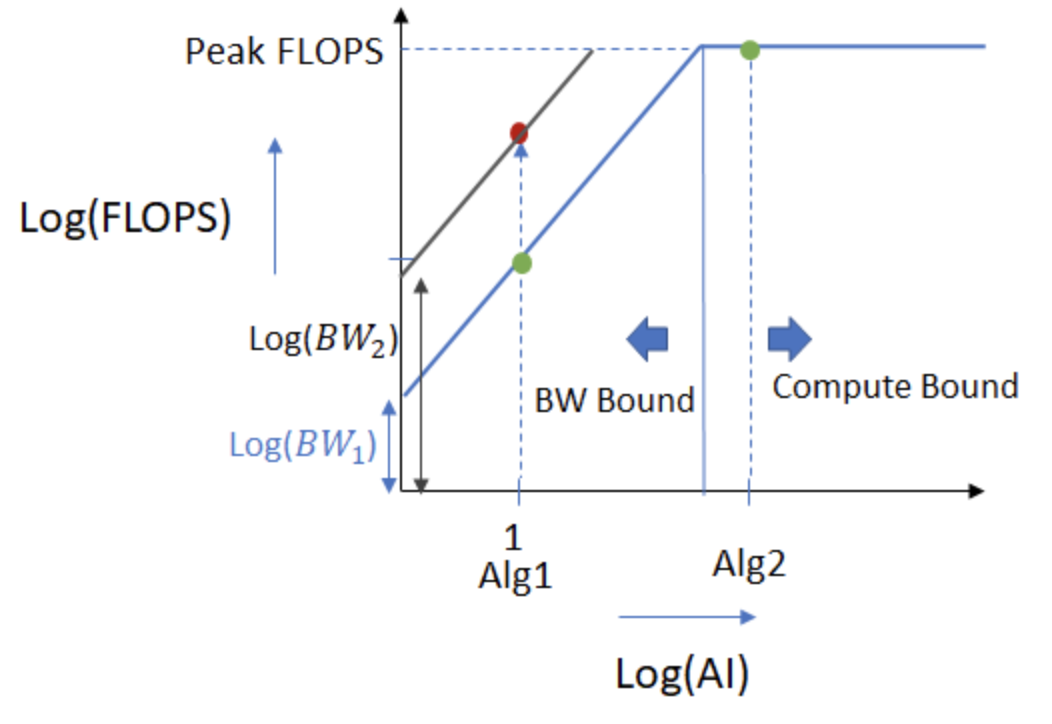
\includegraphics[width=0.8\linewidth]{roofline_plot.png}
    \caption{Roofline Plot for Naive Matrix-Matrix Multiplication}
\end{figure}

\begin{figure}[!htb]
    \centering
    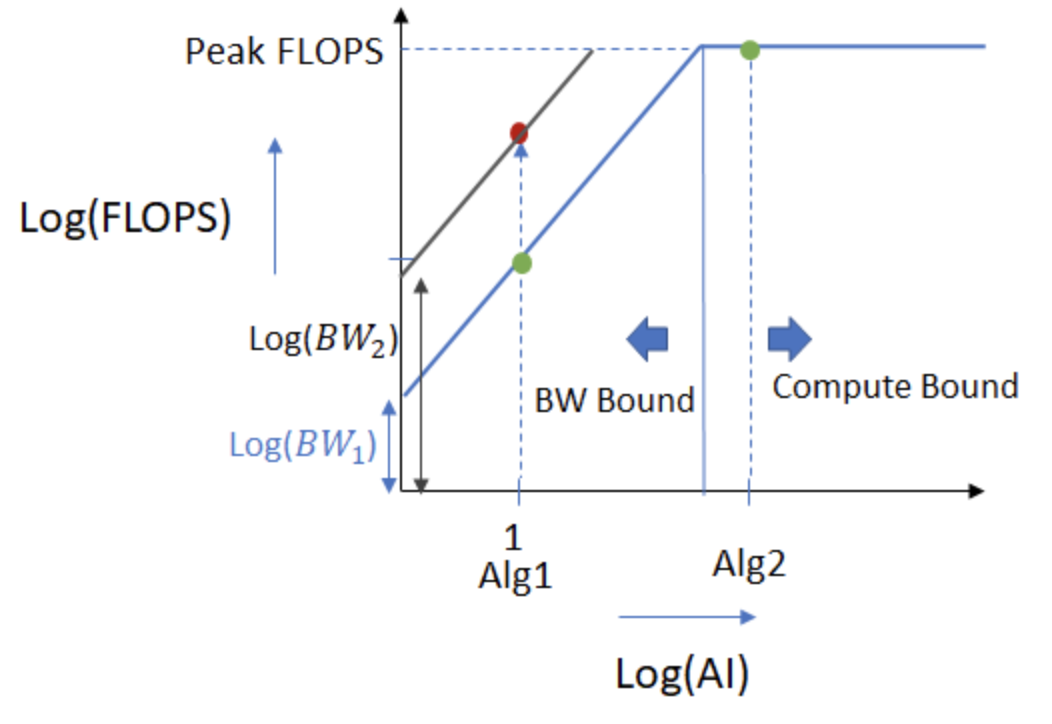
\includegraphics[width=0.8\linewidth]{roofline_plot.png}
    \caption{Roofline Plot for Blocked Matrix-Matrix Multiplication}
\end{figure}


\section{Recursive Matrix-Matrix Multiplication}

\subsection{Results}
\begin{figure}[!htb]
    \centering
    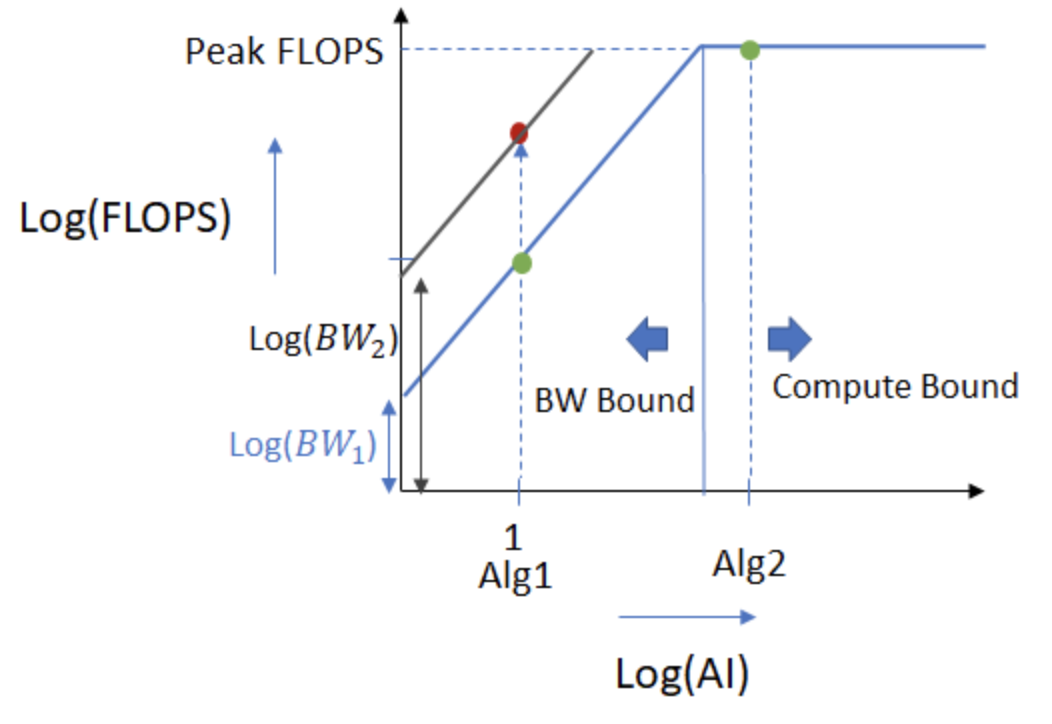
\includegraphics[width=0.8\linewidth]{roofline_plot.png}
    \caption{Roofline Plot for Recursive Matrix-Matrix Multiplication}
\end{figure}

\subsection{Discussion}
\begin{verbatim}
\end{verbatim}

\end{document}
